%%%%%%%%%%%%%%%%%%%%%%%%%%%%%%%%%%%%%%%%%%%%%%%%%%%%%%%%%%%%%%%%%%%%%%%%%%%%%%%%
% simulation.tex: Chapter on MC production:
%%%%%%%%%%%%%%%%%%%%%%%%%%%%%%%%%%%%%%%%%%%%%%%%%%%%%%%%%%%%%%%%%%%%%%%%%%%%%%%%
\chapter{Simulation}
\label{chapter:ldmx:simulation}
%%%%%%%%%%%%%%%%%%%%%%%%%%%%%%%%%%%%%%%%%%%%%%%%%%%%%%%%%%%%%%%%%%%%%%%%%%%%%%%%

\todo[inline]{General description of LDMX software and how it constructs a data processing
    pipeline. Geant4, MadGraph/MadEvent, electronics emulation, and reconstruction.}

LDMX (like many other HEP experiments) uses an intricate software stack in order to realistically and efficiently simulate particle interactions with the detector, emulate the electronics that would be used to measure these interactions, and reconstruct the output of these electronics into physically-understandable variables.
These software tasks are accomplished by a wide swath of different software packages, some of which custom-written for LDMX, most of which written in C++.
This chapter is focused on describing this simulation infrastructure -- focusing particularly on parts of the infrastructure I was involved in -- while also pointing out areas that are expected to remain constant in the presence of data gathered from a real detector.

\section{General Data Process}
One of the core principles helping organize HEP data is the concept of an ``event.''
Events are a bit abstract to define in terms of the physical experiment; however, they are slightly easier to define within the confines of our data processing software.
In essence, each event within the software is independent from one another however they all share a similar structure to the information they hold. A natural example is a data table: a row has the same values in each of its columns as all the other rows. Events behave the same way; however, unlike a data table, the structure of an event can be more intricate than simply a series of values corresponding to different column titles.

While our basic ``unit'' of data is an event, we require many events in order to make statistical conclusions about our data; thus, we have developed a ``event processing framework'' that allows us to unify the various aspects of processing the data held within an event. This data processing framework, colloquially known as ``Framework''

\begin{figure}
    \centering
    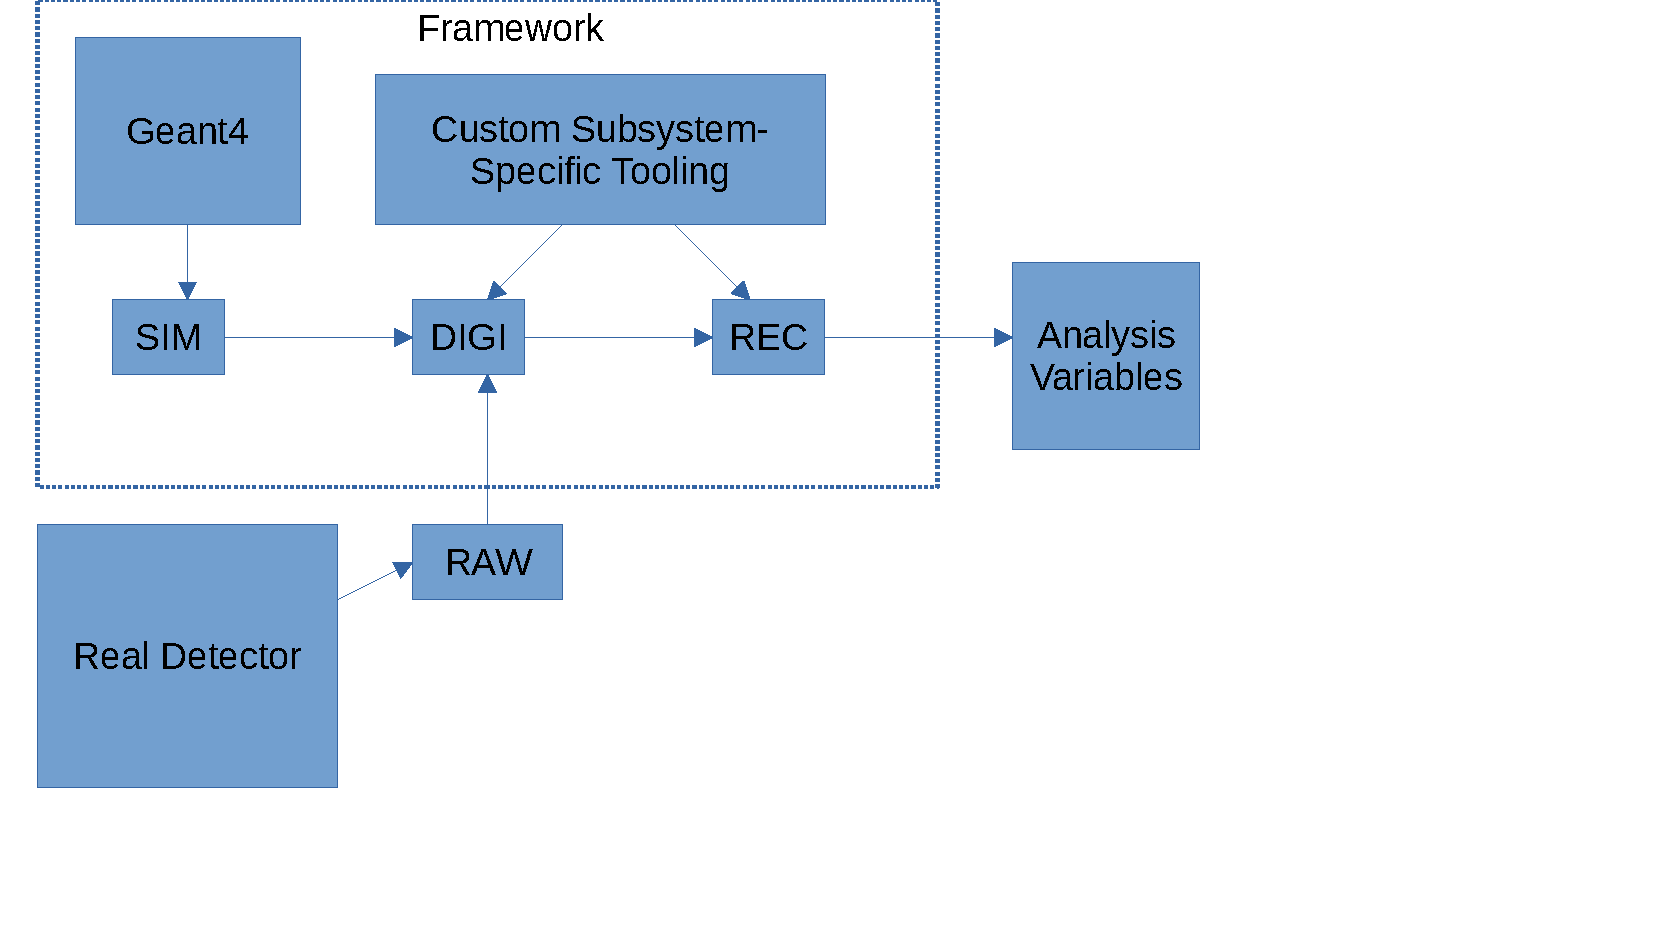
\includegraphics[width=0.9\textwidth]{figures/ldmx/simulation/data-flow.pdf}
    \caption{
        Diagram showing flow of data within LDMX processing.
    }
    \label{fig:ldmx:sim:data-flow}
\end{figure}

\section{Standard Processes}
\todo[inline]{``Backgrounds'' -- version of Geant4 and how it has been configured (broadly).}

\subsection{Biasing and Filtering}
\todo[inline]{Biasing and filtering methodology, configuration for EaT-specific backgrounds.}

\subsection{Validation}
\todo[inline]{Validation of this methodology.}

\section{\gls{dm} Signal}
The particular signal process this analysis channel is looking for is the
production of a dark photon followed by an \emph{invisible} decay. In this
regime, what happens to the dark photon after it is produced is irrelevant
to the analysis since both it and its products are not observable by our
detector.

With this focus in mind, we developed a dark bremsstrahlung simulation method
that allows for the visible particle (the recoiling lepton) to be distributed
according to a full matrix element calculation (via MG/ME) while the incident
particle can have varied energy and be handled by Geant4 directly. This novel
simulation technique allows for the dark bremsstrahlung process to be treated
(from Geant4's perspective) on the same footing as the background processes
while maintaining the precision of a matrix-calculator method.

\subsection{G4DarkBreM}
\todo[inline]{Description of scaling as well as citation to paper.}

\subsection{MadGraph/MadEvent}
\todo[inline]{Detail on MG/ME workspace used to generate DB libraries.}

\subsection{Characterization}
\todo[inline]{Describe how these samples "look"?}

%%%%%%%%%%%%%%%%%%%%%%%%%%%%%%%%%%%%%%%%%%%%%%%%%%%%%%%%%%%%%%%%%%%%%%%%%%%%%%%%
